\documentclass[border=10pt]{standalone}
\usepackage{tikz}
\usepackage{amsmath}

\definecolor{polecol}{RGB}{204,51,51}
\definecolor{gridcol}{RGB}{50,50,80}
\definecolor{ringcol}{RGB}{140,140,160}
\definecolor{annotcol}{RGB}{80,80,80}
\definecolor{stencilA}{RGB}{0,150,130}

\begin{document}
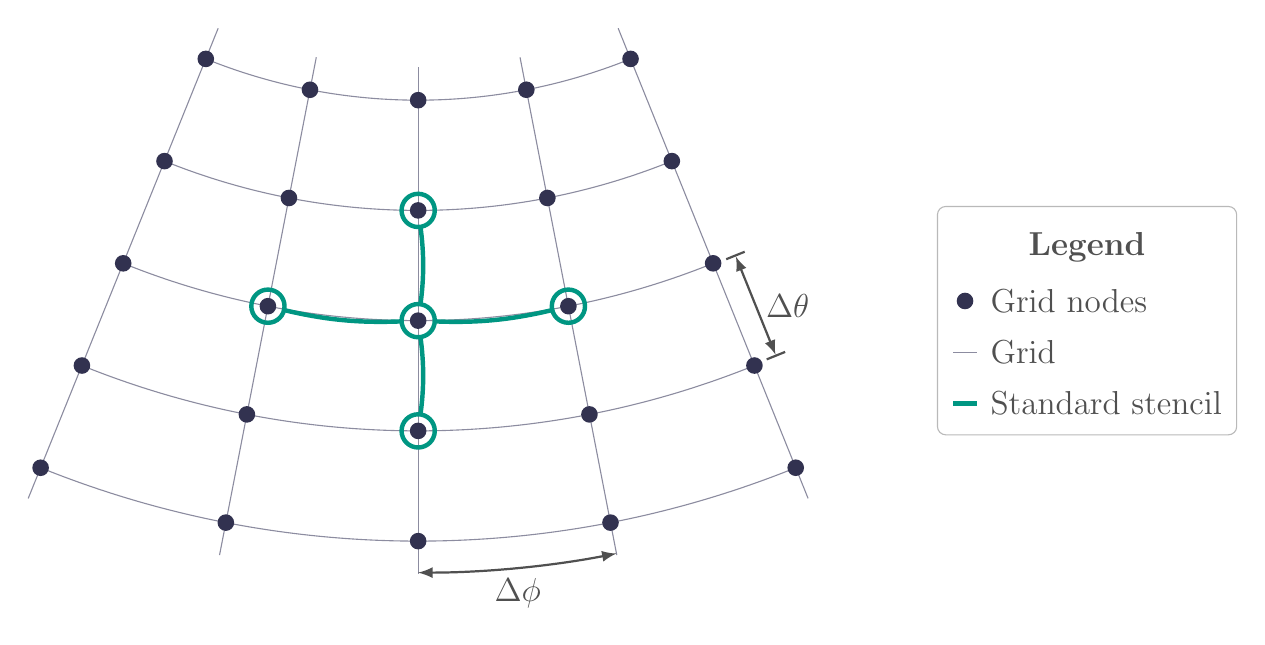
\begin{tikzpicture}[>=latex]

	% --- Parameters ---
	\def\dtheta{1.4}
	\def\Npts{5}           % 5x5 grid
	\def\arcRadius{10.0}   % curvature radius — controls how "spherical" it looks
	\def\halfSpan{22}      % half angular span for 5 longitude lines

	% Grid is centered at row 3, col 3 (1-indexed)
	% Rows go from arcRadius - 2*dtheta to arcRadius + 2*dtheta
	% Cols go from -halfSpan to +halfSpan

	\pgfmathsetmacro{\startAng}{270 - \halfSpan}
	\pgfmathsetmacro{\endAng}{270 + \halfSpan}

	% =============================================
	%  GRID LINES
	% =============================================

	% --- Latitude arcs ---
	\foreach \i in {0,...,\the\numexpr\Npts-1\relax} {
			\pgfmathsetmacro{\r}{\arcRadius + (\i - 2) * \dtheta}
			\draw[ringcol, thin] (\startAng:\r) arc (\startAng:\endAng:\r);
		}

	% --- Longitude lines ---
	\foreach \j in {0,...,\the\numexpr\Npts-1\relax} {
			\pgfmathsetmacro{\ang}{\startAng + \j * 2*\halfSpan / (\Npts - 1)}
			\pgfmathsetmacro{\rBot}{\arcRadius - 2.3*\dtheta}
			\pgfmathsetmacro{\rTop}{\arcRadius + 2.3*\dtheta}
			\draw[ringcol, thin] (\ang:\rBot) -- (\ang:\rTop);
		}

	% =============================================
	%  GRID DOTS
	% =============================================

	\foreach \i in {0,...,\the\numexpr\Npts-1\relax} {
			\foreach \j in {0,...,\the\numexpr\Npts-1\relax} {
					\pgfmathsetmacro{\r}{\arcRadius + (\i - 2) * \dtheta}
					\pgfmathsetmacro{\ang}{\startAng + \j * 2*\halfSpan / (\Npts - 1)}
					\fill[gridcol] (\ang:\r) circle (3pt);
				}
		}

	% =============================================
	%  STENCIL: 5-point at center (row=2, col=2, 0-indexed)
	% =============================================

	% Center
	\pgfmathsetmacro{\rCen}{\arcRadius}
	\pgfmathsetmacro{\angCen}{\startAng + 2 * 2*\halfSpan / (\Npts - 1)}
	\pgfmathsetmacro{\xCen}{\rCen * cos(\angCen)}
	\pgfmathsetmacro{\yCen}{\rCen * sin(\angCen)}

	% North (poleward, row-1)
	\pgfmathsetmacro{\rN}{\arcRadius - \dtheta}
	\pgfmathsetmacro{\xN}{\rN * cos(\angCen)}
	\pgfmathsetmacro{\yN}{\rN * sin(\angCen)}

	% South (equatorward, row+1)
	\pgfmathsetmacro{\rS}{\arcRadius + \dtheta}
	\pgfmathsetmacro{\xS}{\rS * cos(\angCen)}
	\pgfmathsetmacro{\yS}{\rS * sin(\angCen)}

	% East (col+1)
	\pgfmathsetmacro{\angE}{\startAng + 3 * 2*\halfSpan / (\Npts - 1)}
	\pgfmathsetmacro{\xE}{\rCen * cos(\angE)}
	\pgfmathsetmacro{\yE}{\rCen * sin(\angE)}

	% West (col-1)
	\pgfmathsetmacro{\angW}{\startAng + 1 * 2*\halfSpan / (\Npts - 1)}
	\pgfmathsetmacro{\xW}{\rCen * cos(\angW)}
	\pgfmathsetmacro{\yW}{\rCen * sin(\angW)}

	% Circle stencil points
	\draw[stencilA, ultra thick] (\xCen, \yCen) circle (6pt);
	\draw[stencilA, ultra thick] (\xN, \yN) circle (6pt);
	\draw[stencilA, ultra thick] (\xS, \yS) circle (6pt);
	\draw[stencilA, ultra thick] (\xE, \yE) circle (6pt);
	\draw[stencilA, ultra thick] (\xW, \yW) circle (6pt);

	% Stencil arrows
	\draw[stencilA, ultra thick, shorten <=5.5pt, shorten >=5.5pt]
	(\xCen, \yCen) to[bend right=8] (\xN, \yN);
	\draw[stencilA, ultra thick, shorten <=5.5pt, shorten >=5.5pt]
	(\xCen, \yCen) to[bend left=8] (\xS, \yS);
	\draw[stencilA, ultra thick, shorten <=5.5pt, shorten >=5.5pt]
	(\xCen, \yCen) to[bend right=8] (\xE, \yE);
	\draw[stencilA, ultra thick, shorten <=5.5pt, shorten >=5.5pt]
	(\xCen, \yCen) to[bend left=8] (\xW, \yW);

	% =============================================
	%  DISTANCE ANNOTATIONS
	% =============================================

	% Delta theta — right side
	\pgfmathsetmacro{\annotAng}{\startAng + 4 * 2*\halfSpan / (\Npts - 1)}
	\pgfmathsetmacro{\rA}{\arcRadius}
	\pgfmathsetmacro{\rB}{\arcRadius + \dtheta}
	\pgfmathsetmacro{\xA}{\rA * cos(\annotAng) + 0.3 * cos(\annotAng + 90)}
	\pgfmathsetmacro{\yA}{\rA * sin(\annotAng) + 0.3 * sin(\annotAng + 90)}
	\pgfmathsetmacro{\xB}{\rB * cos(\annotAng) + 0.3 * cos(\annotAng + 90)}
	\pgfmathsetmacro{\yB}{\rB * sin(\annotAng) + 0.3 * sin(\annotAng + 90)}
	\draw[thick, |<->|, annotcol] (\xA, \yA) -- (\xB, \yB)
	node[midway, right, font=\large] {$\Delta\theta$};

	% Delta phi — arc at bottom
	\pgfmathsetmacro{\rDp}{\arcRadius + 2*\dtheta + 0.4}
	\pgfmathsetmacro{\angDpL}{\startAng + 2 * 2*\halfSpan / (\Npts - 1)}
	\pgfmathsetmacro{\angDpR}{\startAng + 3 * 2*\halfSpan / (\Npts - 1)}
	\draw[thick, <->, annotcol]
	(\angDpL:\rDp) arc (\angDpL:\angDpR:\rDp)
	node[midway, below, font=\large] {$\Delta\phi$};

	% =============================================
	%  LEGEND (to the right, vertically centered)
	% =============================================

	% Compute right edge of grid
	\pgfmathsetmacro{\gridRightX}{(\arcRadius + 2*\dtheta) * cos(\endAng)}

	% Legend entries: 3 items, each 0.65 apart, total height = 2*0.65 = 1.3
	% Plus title row: total ~2.1, center around y = yCen
	\pgfmathsetmacro{\legX}{\gridRightX + 1.8}

	\begin{scope}[shift={(\legX, \yCen + 1.45)}]

		% Title
		\node[anchor=north, font=\large\bfseries, annotcol] at (1.9, -0.2) {Legend};

		% Grid nodes
		\fill[gridcol] (0.35, -1.2) circle (3pt);
		\node[anchor=west, font=\large, annotcol] at (0.55, -1.2)
		{Grid nodes};

		% Grid lines
		\draw[ringcol, thin] (0.2, -1.85) -- (0.5, -1.85);
		\node[anchor=west, font=\large, annotcol] at (0.55, -1.85)
		{Grid};

		% Standard Stencil
		\draw[stencilA, ultra thick] (0.2, -2.5) -- (0.5, -2.5);
		\node[anchor=west, font=\large, annotcol] at (0.55, -2.5)
		{Standard stencil};

		% Bounding box with 0.2 margins
		\draw[anchor=west,annotcol!40, rounded corners=3pt]
		(0, 0) rectangle (3.8, -2.9);
	\end{scope}

\end{tikzpicture}
\end{document}
